\documentclass[11pt,letterpaper]{article}
\usepackage[T1]{fontenc}
\usepackage[utf8]{inputenc}
\usepackage{lmodern}
\usepackage[margin=0.85in]{geometry}
\usepackage{graphicx,booktabs,tabularx,longtable,array}
\usepackage{xcolor,microtype,enumitem,fancyhdr}
\usepackage{amsmath}
\usepackage[breaklinks=true,colorlinks=true,linkcolor=teal,citecolor=teal,urlcolor=teal]{hyperref}
\definecolor{teal}{RGB}{23,107,120}
\setlength{\parindent}{0pt}
\setlength{\parskip}{6pt}
\setlength{\headheight}{15pt}
\setlength{\emergencystretch}{2em}
\setlist{nosep,leftmargin=*}
\setlist[description]{style=nextline,leftmargin=0pt,labelwidth=0pt,labelsep=0pt}
\widowpenalty=10000
\clubpenalty=10000
\pagestyle{fancy}
\fancyhf{}
\fancyhead[L]{\small\textcolor{teal}{Poker Agent Lab}}
\fancyhead[R]{\small Experimental report}
\fancyfoot[C]{\small\thepage}
\newcolumntype{Y}{>{\raggedright\arraybackslash}X}
\makeatletter
\newcommand{\inputtable}[1]{\@@input #1 }
\makeatother
\graphicspath{{figures/}}
\title{\textbf{Poker Agent Lab}\\[5pt]\large Book-inspired policies, reproducible experiments,\\and comparison with open-source poker projects}
\author{Repository owner: \texttt{msnouri}}
\date{November 11, 2026}

\begin{document}
\maketitle
\begin{abstract}
We implement 80 heuristic poker policies in 16 conceptual families and test
them in ordinary no-limit Texas Hold'em. Each candidate receives 500 direct
self-play hands and 500 matched-opponent screening hands. Twenty-five
shortlisted policies receive 2,000 fresh validation hands each, and eight
finalists are evaluated in 3,072 eight-player tournaments. S55, an equity
realization and pot-control policy, has the largest mean score across the
three synthetic tournament fields, without separating statistically from
every finalist. A subsequent frozen-policy comparison covers 70,000 heads-up
hands, 35,000 eight-player cash hands, and 896 tournaments against seven
adapted Neuron Poker example policies. S55 leads those tournament
comparisons but loses substantially against aggressive examples in heads-up
cash play. No pretrained DQN or CFR model is benchmarked. The evidence
supports a format-specific research baseline, not general superiority or
competition readiness.
\end{abstract}

\section{Objective and evidence boundary}
The goal is to create an offline poker agent and evaluate strategy ideas in a
controlled setting, with possible application to a bot competition such as
Sequoia's No Limit event~\cite{competition}. The experiments assume ordinary
two-hole-card no-limit Texas Hold'em. The actual event variant and Agent
interface are supplied at the event, so the present implementation is not a
verified submission.

The 80 candidates are original numerical implementations inspired by selected
book concepts. They are neither 80 independently trained models nor 80
complete strategies prescribed by the authors. Similarly, an organization,
game engine, training framework, and trained playing policy are different
comparison targets. Results below distinguish source inspection from actual
matches.

\section{Source material and policy construction}
\subsection{Book review}
Relevant instructional sections were reviewed from Hellmuth's
\emph{Play Poker Like the Pros}~\cite{hellmuth}, Brokos's \emph{Play Optimal
Poker 2: Range Construction}~\cite{brokos}, and Dangel's \emph{Poker
Poker}~\cite{dangel}. Hellmuth contributes starting-hand discipline,
opponent tendencies, selective aggression, and trapping. Brokos contributes
equity realization, mixed ranges, protection, semi-bluffing, leverage,
shallow stacks, and tournament chip valuation. Dangel primarily treats older
high-low and limit games; only general betting and expected-value concepts
are adapted. His variant-specific probability tables are not reused.

The fourth attachment, Carol Lynne's \emph{Slow-Play (Poker Night 2)}, is
fiction rather than an instructional poker book and is excluded.

\subsection{Sixteen families and five variants}
Table~\ref{tab:families} maps the policy families to their conceptual
sources. Within each family, five variants change opening width, value
thresholds, calling margin, bet size, and eligible bluff/risk settings.
These are structured parameter packages, so a result cannot be attributed
causally to one parameter. Exact values for all 80 policies are tracked in
\texttt{poker\_lab/strategies.csv}.

\begin{table}[htbp]
\centering\small
\caption{Policy families. Attribution is conceptual; numerical settings are original experimental choices.}
\label{tab:families}
\begin{tabularx}{\linewidth}{@{}p{0.95in}Y Y@{}}
\toprule IDs & Mechanism & Conceptual source \\\midrule
\inputtable{tables/families.tex}
\bottomrule
\end{tabularx}
\end{table}

\subsection{Information and decision model}
The acting policy receives its own hole cards, the exposed board, public
action statistics, position, stack/pot quantities, and legal action bounds.
It receives neither actual opponent hole cards nor future board cards.
PokerKit~\cite{pokerkit} handles legal game transitions, all-ins, side pots,
ties, and settlement. Each simulated hand checks chip conservation.

Preflop equity is estimated with 4,000 seeded deals per each of 169 starting
hand classes against one through seven uniformly random opponents. Opening
percentiles weight the 1,326 distinct two-card combinations. Postflop equity
uses 48 sampled unknown holdings and runouts. If $W$ is the sum of pot shares
won over $N=48$ simulations, the implementation returns
\begin{equation}
\widehat{e}=\frac{W+1}{N+2}.
\end{equation}
The weak smoothing prior avoids exact zero/one estimates from few samples.
Independent local seeds govern dealing, mixed policy choices, and equity
sampling. The same public information set gives the same equity sample.
eval7 performs hand evaluation~\cite{eval7}.

Pot odds use the call cost $c$ and current pot $P$, including the bet faced:
\begin{equation}
e_{\mathrm{break\text{-}even}}=\frac{c}{P+c}.
\end{equation}
Realization, public betting pressure, board texture, draw features, stack
depth, and heuristic margins modify this threshold. Uniform random-hand
equity is \emph{not} a reconstructed conditional opponent range. The
polarized policy is not a GTO solution, and no multi-street search or
exploitability guarantee is implemented.

\section{Initial experimental design}
\begin{table}[htbp]
\centering\small
\caption{Completed initial evaluation. A player-hand and a table-hand are different units.}
\begin{tabularx}{\linewidth}{@{}p{1.25in}Y@{}}
\toprule Phase & Scope and controls \\\midrule
Direct self-play & 80 policies $\times$ 500 hands = 40,000 player-hands, or 5,000 table-hands. Groups of eight are redrawn every eight hands; seats rotate. \\
Matched gauntlet & 80 policies $\times$ 500 hands = 40,000 table-hands. Each candidate faces the same seven baseline policies using common shuffled deals; each seat occurs 62 or 63 times. \\
Fresh validation & Top eight from each initial test plus each family's best gauntlet representative: 25 unique candidates, 2,000 new hands each = 50,000 table-hands. \\
Tournaments & Eight finalists $\times$ 128 tables $\times$ three fields = 3,072 sit-and-gos and 529,966 table-hands. \\
\bottomrule
\end{tabularx}
\end{table}

Reset-stack hands start with 2,000 chips per player and blinds 10/20, without
rake. The baseline population is a restricted collection of original
heuristics related to the candidate architecture, not an independent
representative sample of strong poker opponents. Full field definitions
are in \texttt{poker\_lab/baseline\_fields.json}.

Tournament stacks persist. Players start with 2,000 chips; big blinds follow
$20,30,40,60,100,150,200,300$ with 25 hands per level. Tables end with one
survivor or after 200 hands. The assumed payouts are 50/30/20 points for the
top three. Survivors at the cap receive exact ICM expected values of the
remaining places. Simultaneous eliminations use start-of-hand stacks;
exact ties split the affected place points.

For a remaining stack vector $\mathbf{s}$, ICM recursively weights the chance
of first place by $s_i/\sum_j s_j$, removes that player, and applies the
remaining payouts to the residual stacks. This calculation is exact for
cap scoring. Policy decisions use only a small risk-margin approximation,
not full ICM action optimization.

\section{Initial results and selection uncertainty}
The direct self-play leader is S65; the matched 500-hand gauntlet leader is
S40. On fresh validation, S55 leads. This disagreement demonstrates the
weakness of choosing the largest profit from one short run.

\begin{figure}[htbp]
\centering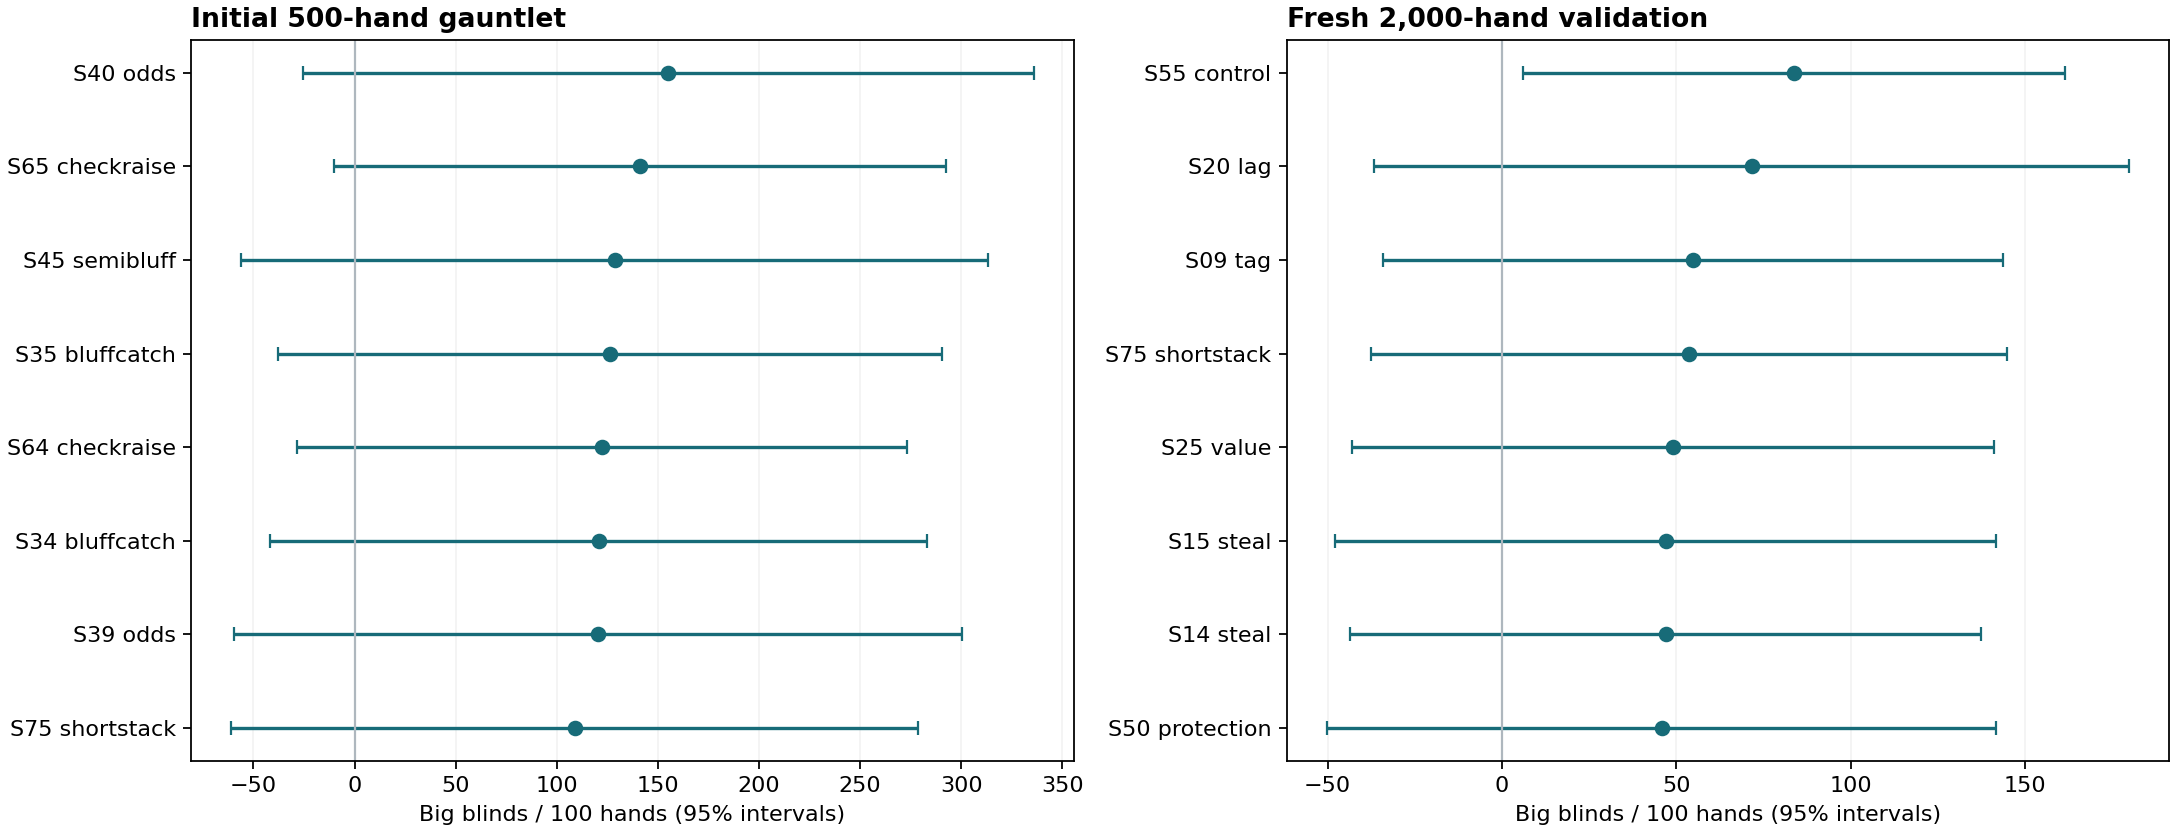
\includegraphics[width=\linewidth]{chip_comparison.png}
\caption{Top chip-return estimates in initial gauntlet screening and fresh validation. Ordinary 95\% intervals are shown; the initial 80-way selection is not corrected.}
\label{fig:chips}
\end{figure}

S55's equally weighted mean across the three tournament fields is 16.30
points per table, with an ordinary 95\% interval of $[14.14,18.46]$.
Table~\ref{tab:rankings} lists the finalists. Overall uncertainty uses each
matched seed's average across the three fields as one observation, retaining
cross-field dependence. Paired differences apply a Bonferroni correction
covering all 28 finalist pairs. S55 does not separate from every finalist.

\begin{table}[htbp]
\centering\small
\caption{Initial tournament finalists, equally weighting mixed, tight, and aggressive fields.}
\label{tab:rankings}
\begin{tabular}{@{}llrr@{}}
\toprule Policy & Family & Mean points & Ordinary 95\% interval \\\midrule
\inputtable{tables/original_rankings.tex}
\bottomrule
\end{tabular}
\end{table}

\begin{figure}[htbp]
\centering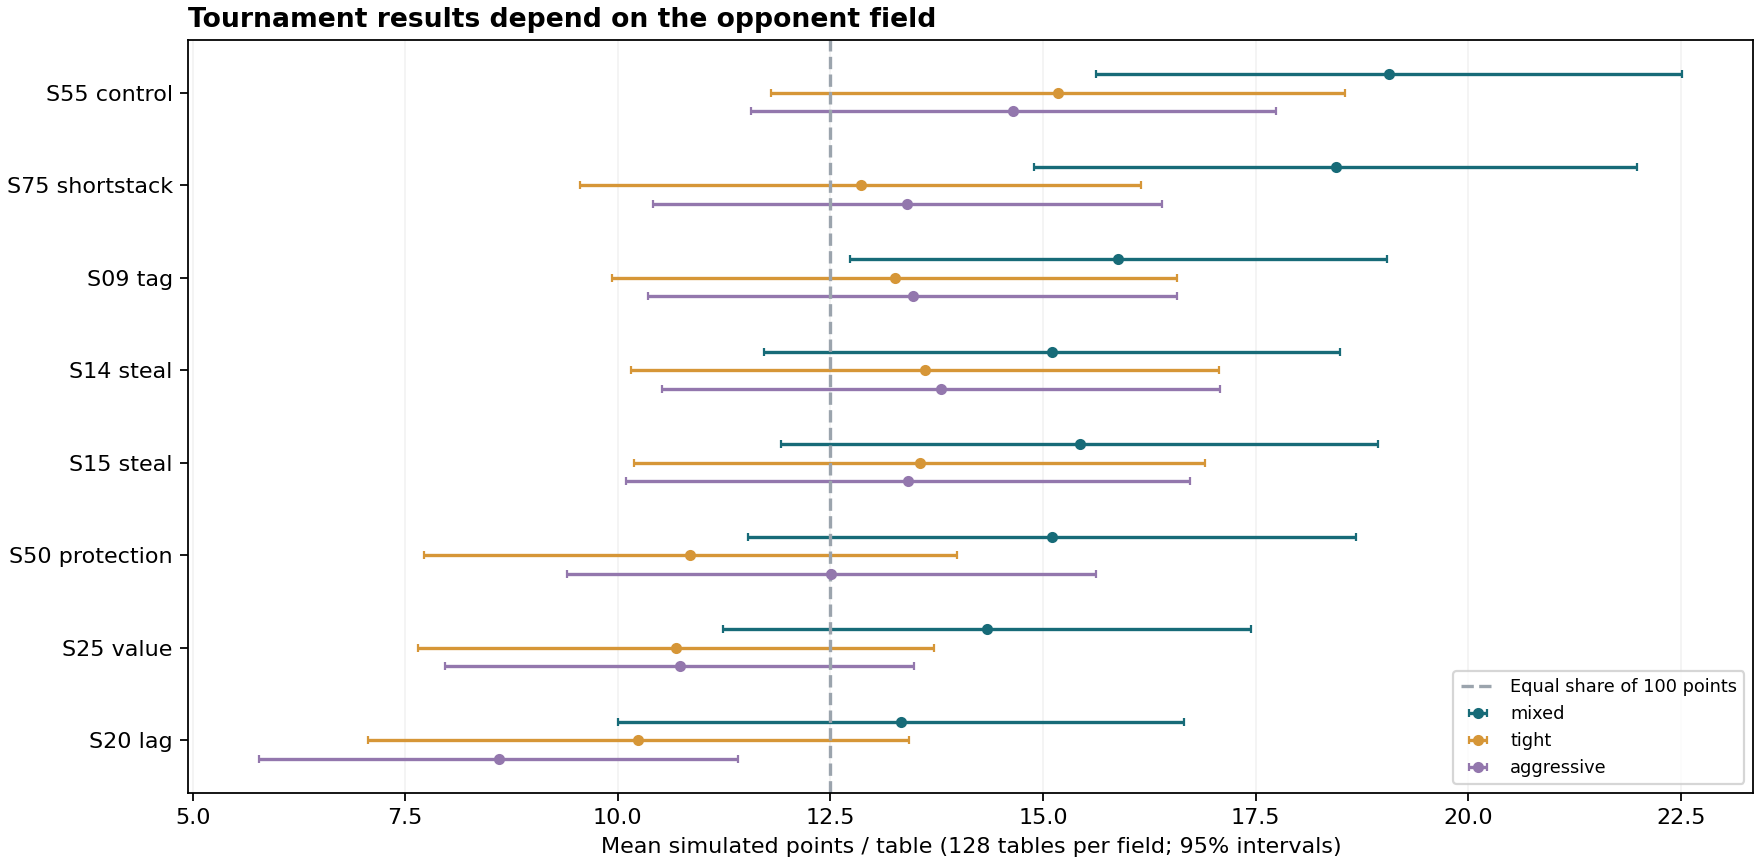
\includegraphics[width=0.95\linewidth]{tournament_comparison.png}
\caption{Initial tournament results by opponent field. The 12.5-point line denotes an equal share of 100 available points, not an expected score for any named baseline.}
\end{figure}

S55 is variant five of the realization/pot-control family.
Table~\ref{tab:s55} records its principal numerical settings. The policy and
equity source remain frozen during the external comparison.
\begin{table}[htbp]
\centering\small
\caption{Selected S55 parameters; exact machine-readable configuration is tracked.}
\label{tab:s55}
\begin{tabular}{@{}lr@{}}
\toprule Parameter & Value \\\midrule
\inputtable{tables/s55_parameters.tex}
\bottomrule
\end{tabular}
\end{table}

\section{Review of the supplied GitHub links}
\begin{description}[style=nextline]
\item[\texttt{uoftcprg}]
A research organization providing PokerKit, NoRegret, datasets, and other
tools~\cite{uoftcprg,noregret}. PokerKit already serves as this project's
engine. NoRegret is a computational game-solving framework with examples
such as Kuhn and Leduc poker, not one pretrained eight-player opponent.
\item[\texttt{apehex/awesome-poker}]
A curated resource directory~\cite{awesome}. It points to engines, bots,
papers, and platforms. The directory itself cannot play a match; its
entries require separate selection and evaluation.
\item[\texttt{HarperJonesGPT/PokerGPT}]
A six-player cash-game assistant using screen/OCR interaction and a live
GPT-4 API call~\cite{pokergpt}. It does not run unchanged in an offline event
sandbox. No match was played, and its strength relative to S55 is unknown.
\item[\texttt{masterai-top/cfr-poker-ai-masterai}]
A heads-up no-limit CFR/ReBeL-style research stack~\cite{masterai}.
The inspected deployment configuration points to
\texttt{./weights/value\_net.net}, absent from its complete inspected tree.
Two \texttt{regrets.*.i} files are present, but were not established to be a
complete compatible playing policy. Its benchmark document explicitly
identifies the old headline win rates as unreproduced project reports
\cite{masteraibench}. No playing-strength result against it is claimed.
\item[\texttt{dickreuter/neuron\_poker}]
A training environment with example random/equity policies and DQN
training/loading code~\cite{neuron}. The loader expects architecture JSON
and H5 weights generated by training; no trained weight artifact appears
in the complete inspected repository tree. Seven example-policy
configurations are tested below. No trained DQN is tested.
\item[\texttt{github.com/topics/poker-game}]
A discovery page spanning game engines, interfaces, and AI projects
\cite{topic}. It is not a single policy. Its visible listings were reviewed,
not every linked repository benchmarked.
\end{description}

\subsection{Source snapshot and artifact availability}
Recursive GitHub inventories were not truncated. The inspected Neuron Poker
tree has 53 files and tree identifier
\texttt{242741ca6bcbdbebccacef1caee2bbb7273355f7}. The inspected MasterAI tree
has 689 files and tree identifier
\texttt{98378370397843817d1cef2e392dc49d6c72672a}. These are Git
\emph{tree} identifiers, not claimed commit hashes. Full inventories and
individual file blob hashes are tracked in
\texttt{github\_comparison/review\_inventory.json}.

Source inspection establishes architecture, dependencies, and artifact
availability. It does not establish playing strength. A CFR algorithm name,
neural architecture, or repository star count cannot substitute for a
compatible trained policy and controlled evaluation.

\section{External example-policy benchmark}
\subsection{Preserved logic and adapter changes}
The original random and equity-threshold action method bodies execute
unchanged. Only their Gym Enum import is removed; the original Enum is
injected. The six threshold pairs are the upstream genetic-improvement
initialization values: $(0.1,0.2)$ through $(0.6,0.7)$, interpreted as minimum
call and bet equity. They were not tuned against S55.

The native Gym engine is replaced by PokerKit legality and settlement.
Both sides receive our shared equity feature: the existing preflop asset
and 48 postflop samples. Thus the experiment isolates much of the decision
logic but does not compare the full native equity pipelines. Upstream
half-pot, pot, and twice-pot actions retain their additional-contribution
interpretation. Only legal standard no-limit targets are offered;
fractional chip contributions round down. All-in uses the maximum legal
target. The native Gym per-player raise cap is not imposed.

These are \textbf{adapted example-policy tests}, not a victory claim over
the full Neuron Poker stack or a pretrained neural model.

\subsection{Match formats and sample units}
\begin{itemize}
\item \textbf{Heads-up cash:} 5,000 independent shuffled deals per opponent,
each played from both seats: 10,000 hands per configuration, 70,000 total.
The statistical unit is the average return over the two seat-swapped hands.
\item \textbf{Eight-player cash:} 5,000 independent table-hands per opponent,
35,000 total, with rotating seats and reset 2,000-chip stacks. Each table
has four independent S55 copies and four independent external copies.
The sample unit is one table-hand's mean return per S55 copy.
\item \textbf{Eight-player tournaments:} 128 tables per opponent, 896 total,
covering 138,187 table-hands. The same four-versus-four composition is used.
The sample unit is the table's cohort-average points per S55 copy.
\end{itemize}

Copies do not coordinate or share hidden cards or policy state. Averaging
their scores is an evaluation operation, not agent cooperation. Initial
stacks, blind schedule, assumed payouts, cap scoring, and rake conventions
match the preceding research design. Match seeds differ from the original
screening and validation phases. No 1~ms deadline folds are imposed.

\subsection{Metric and uncertainty}
For returns $x_i$ in big blinds over $n$ independent sample units, the chip
rate and ordinary interval are
\begin{align}
\widehat{\mu}_{100}&=100\bar{x},\\
\mathrm{CI}_{95}&=100\left(\bar{x}\pm t_{n-1,0.975}
\frac{s_x}{\sqrt{n}}\right).
\end{align}
For tournaments the same mean/standard-error calculation applies directly
to cohort-average points, without the factor 100. Four bots from one table
are not treated as four independent samples. Simultaneous bounds across all
21 metric/configuration comparisons use critical probability
$1-0.05/(2\times21)$ rather than $0.975$.

\subsection{Results}
\begin{table}[htbp]
\centering\small
\caption{Frozen S55 against adapted Neuron Poker example policies. Positive chip rates favor S55; tournament parity is 12.5 points per bot.}
\label{tab:external}
\begin{tabular}{@{}lrrr@{}}
\toprule Opponent & Heads-up bb/100 & 8-player cash bb/100 & Tournament points/bot \\\midrule
\inputtable{tables/external_results.tex}
\bottomrule
\end{tabular}
\end{table}

\begin{table}[htbp]
\centering\small
\caption{Ordinary 95\% intervals for selected external comparison metrics. Simultaneously corrected intervals are included in the figure and tracked CSV.}
\begin{tabular}{@{}lll@{}}
\toprule Opponent & Heads-up bb/100 interval & Tournament points/bot interval \\\midrule
\inputtable{tables/external_intervals.tex}
\bottomrule
\end{tabular}
\end{table}

\begin{figure}[htbp]
\centering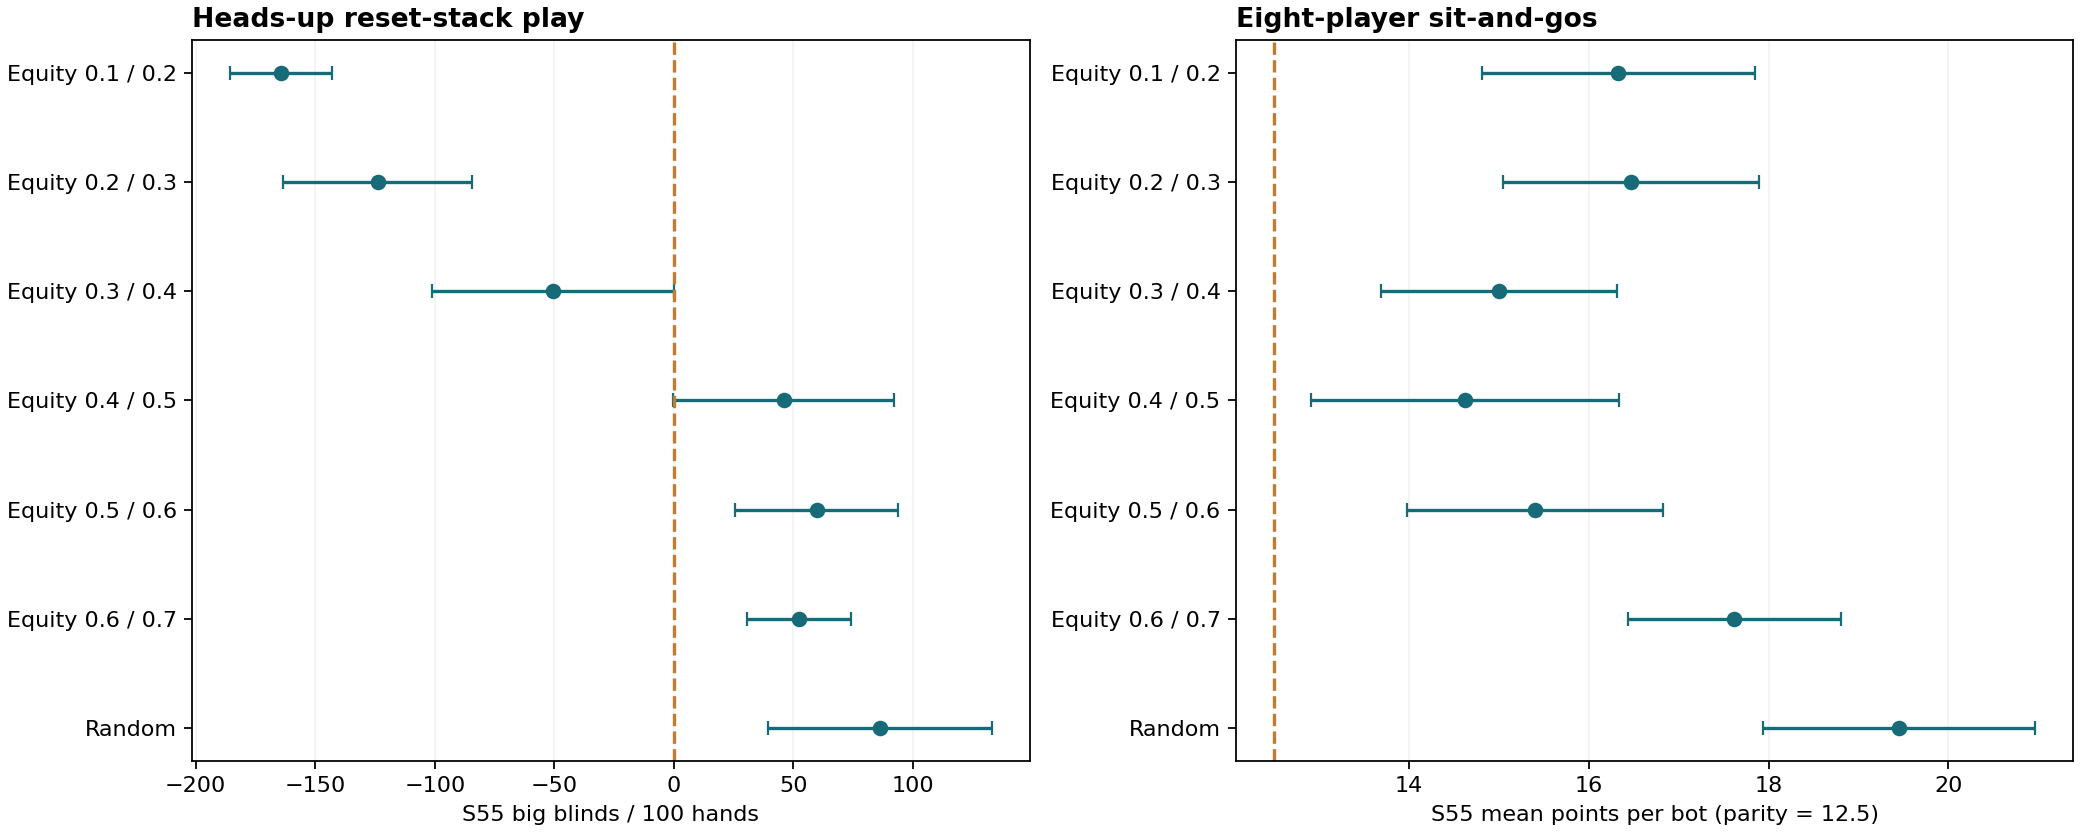
\includegraphics[width=\linewidth]{external_comparison.png}
\caption{External-policy results with simultaneous 95\% intervals corrected across all 21 reported metric/configuration comparisons.}
\label{fig:external}
\end{figure}

Against the most aggressive threshold example, S55 loses 164.28 big blinds
per 100 heads-up hands, with ordinary interval $[-177.96,-150.59]$.
Against random play, it earns $+86.04$ bb/100. In the eight-player tournament
tests, mean S55 points per bot range from 14.63 to 19.45. All seven
tournament configurations remain above the 12.5 parity reference under the
simultaneous correction. These findings concern the specified four-versus-four
composition, adapter, and payout assumptions.

\section{Interpretation and limitations}
S55 is useful as a measured baseline for the assumed eight-player tournament,
but the evidence does not support calling it a strong general poker model.
Its initial related-opponent success does not carry over uniformly to the
external tests.

Code inspection suggests that narrow all-in calling rules and the
random-opponent equity assumption contribute to the heads-up weakness.
The policy does not fully widen its calling response when an opponent
repeatedly shoves weak holdings. Repeated folds surrender blinds heads-up,
while survival and avoiding other players' confrontations have value under
top-three tournament payouts. This is an interpretation, not a causal
ablation study.

Material limitations are:
\begin{enumerate}
\item Initial 500-hand rankings have substantial sampling uncertainty and
winner's curse. Fresh validation selects finalists and therefore is not
untouched final confirmation.
\item Opponent fields are synthetic and restricted. Four-versus-four external
tests do not establish performance at tables of eight independently designed
strong bots.
\item Uniform-hand equity, simple betting-pressure penalties, and 48 postflop
samples do not reconstruct full opponent ranges. No equilibrium strategy,
multi-street solver, or learned policy is implemented.
\item No trained DQN/CFR opponent was benchmarked. Missing compatible weights
and interfaces prevent broad comparisons with the named research projects.
\item Cash chip profit and tournament points measure different objectives.
Heads-up and multiplayer results must remain separate.
\item Recorded timings do not enforce the competition deadline. Original
isolated S55 measurements covered 1,305 decisions, including 477 postflop;
cold-cache p99 was approximately 0.288~ms with no over-1~ms samples in that
measurement. Initialization and state conversion were excluded, so this is
not sandbox certification.
\end{enumerate}

The official event rules describe eight-bot sit-and-gos, a 200-hand cap,
2,000-chip starts, 10/20 starting blinds, and 25-hand levels. They require
offline operation and a 1~ms decision deadline, with the variant and SDK
provided at the build phase~\cite{competition}. Ordinary two-card Hold'em,
the complete blind schedule, and 50/30/20 payouts remain our explicit
research assumptions.

The next research priorities are opponent-conditioned ranges, better
format-specific preflop/all-in responses, and frozen-policy evaluation
against independently trained checkpoints. No claim of superiority should
be based solely on algorithm labels or undocumented win percentages.

\section{Implementation, verification, and reproduction}
\subsection{Repository layout}
\begin{description}[font=\normalfont\ttfamily]
\item[report/] This LaTeX source, compiled PDF, figures, and CSV-driven tables.
\item[poker\_lab/pokerlab/] Agent, strategy registry, engine wrapper, equity
asset generator, experiment runner, analysis, and JSON-lines interface.
\item[poker\_lab/results/] Initial screening, self-play, validation,
tournament records, timing, settings, and source hashes.
\item[github\_comparison/] External policy adapter, pinned source downloader,
raw hand/table results, simultaneous intervals, and repository inventories.
\item[poker\_lab/tests/] Eight checks covering registry uniqueness, equity
sanity, determinism, information boundaries, independent evaluator agreement,
known side pots/ties, ICM, and all policies on varied short stacks.
\end{description}

The original tests include 400 random showdown comparisons between eval7
and Treys~\cite{treys}, and 80 varied-stack strategy hands. The external
adapter's upstream source blobs were checked, and the S55 source hash was
confirmed unchanged. The source downloader pins individual Git blobs rather
than a moving branch.

\subsection{Commands}
Use Python 3.12+ and the tracked dependency versions. From the repository root:
\begin{verbatim}
python3 -m venv .venv
source .venv/bin/activate
python -m pip install -r requirements.txt
make test
make report
\end{verbatim}
To rerun the initial experiment:
\begin{verbatim}
cd poker_lab
python -m pokerlab.experiment --stage all --hands 500 \
  --validation-hands 2000 --tables 128 --workers 8
python -m pokerlab.analyze
\end{verbatim}
To rerun the external example-policy tests from the repository root:
\begin{verbatim}
python github_comparison/download_sources.py
PYTHONHASHSEED=0 python github_comparison/benchmark.py \
  --deals 5000 --tables 128 --workers 8
python github_comparison/build_report.py
\end{verbatim}
\texttt{make report} regenerates the numerical LaTeX tables from recorded
CSVs and compiles the source twice; it does not rerun matches. The source,
figures, and PDF are tracked together. Raw outcomes are seeded; wall times
and numerical presentation may vary by platform.

No uploaded book or extracted full text is distributed. General-purpose
dependencies are installed separately, and external example source is
downloaded separately with its license. No participant repository was copied
into the original agent. No external API is used during gameplay, no poker
client is automated, and no competition submission is made by these scripts.

\clearpage
\begin{thebibliography}{99}\small
\bibitem{hellmuth} P. Hellmuth Jr. \emph{Play Poker Like the Pros}.
Reviewed supplied EPUB, especially chapters 3--4 and 6; chapter 7 for
tournament context.
\bibitem{brokos} A. Brokos. \emph{Play Optimal Poker 2: Range Construction}.
2020. Reviewed chapters 1--6 and chapter 11, especially printed
pp. 304 and 315--318.
\bibitem{dangel} P. N. Dangel. \emph{Poker Poker}. 1977.
Reviewed chapters 5--8, especially printed pp. 132--134, 163--164,
and 192--193.
\bibitem{competition} Sequoia Capital. \emph{No Limit: Official Rules}.
\url{https://pokerbot.sequoiacap.com/rules.html}. Accessed November 11, 2026.
\bibitem{pokerkit} UOFTCPRG. \emph{PokerKit}.
\url{https://github.com/uoftcprg/pokerkit}.
\bibitem{eval7} Julian Andrews et al. \emph{eval7}.
\url{https://github.com/JulianAndrews/pyeval7}.
\bibitem{treys} I. Hendley et al. \emph{Treys}.
\url{https://github.com/ihendley/treys}.
\bibitem{uoftcprg} Universal, Open, Free, and Transparent Computer Poker
Research Group. GitHub organization. \url{https://github.com/uoftcprg}.
\bibitem{noregret} UOFTCPRG. \emph{NoRegret}.
\url{https://github.com/uoftcprg/noregret}.
\bibitem{awesome} apehex. \emph{Awesome Poker}.
\url{https://github.com/apehex/awesome-poker}.
\bibitem{pokergpt} HarperJonesGPT. \emph{PokerGPT}.
\url{https://github.com/HarperJonesGPT/PokerGPT}.
\bibitem{masterai} masterai-top. \emph{cfr-poker-ai-masterai}.
\url{https://github.com/masterai-top/cfr-poker-ai-masterai}.
\bibitem{masteraibench} masterai-top. \emph{Benchmark Reporting Protocol}.
\url{https://github.com/masterai-top/cfr-poker-ai-masterai/blob/main/BENCHMARKS.md}.
\bibitem{neuron} N. Dickreuter. \emph{Neuron Poker}.
\url{https://github.com/dickreuter/neuron_poker}.
\bibitem{topic} GitHub. \emph{poker-game topic}.
\url{https://github.com/topics/poker-game}.
\end{thebibliography}
\end{document}
